\documentclass[11pt]{article}
\usepackage[margin=1in]{geometry}
\usepackage{amsmath,amssymb,booktabs,hyperref}
\usepackage{pgfplots}\pgfplotsset{compat=1.18}
\usepackage[numbers,sort&compress]{natbib}
\title{The Homology Cliff is Cross-Family, Not Within-Family: Pfam Partition of Distant False Alarms and Mapper Topology of the Toxin Manifold}
\author{Santiago Maniches\thanks{ORCID 0009-0005-6480-1987. TOPOLOGICA LLC.}}
\date{April 12, 2026 (v1.1; figure erratum 2026-06-16)}
\begin{document}
\maketitle
\begin{abstract}
We partition the distant-stratum false alarms of frozen ESM-2 t30 cosine $k$-NN retrieval by Pfam family membership. At $R{=}1000$ $k{=}25$ seed 20260410, 41 distant-stratum proteins receive a positive prediction while the true label is negative. Of these, 20 are evaluable (both query and at least one positive-voting panel member carry Pfam annotations); 21 are excluded due to missing annotations on the query or all positive-voting neighbors. Of the 20 evaluable cases, \textbf{zero} share any Pfam identifier with the neighbors who voted them positive. By Wilson 95\% confidence interval on a 20/20 result, the population within-family rate is at most $17\%$. This is consistent with cross-family failures dominating the cliff in this dataset, and inconsistent with the within-family distant-homology hypothesis as the primary mechanism. Complementary Mapper decomposition (149 nodes, 6 all-positive, positive class spatially localized on PCA lens) shows positives cluster densely; the cross-family cliff failures are retrievals from this cluster applied to queries that happen to lie near the cluster periphery in cosine space for reasons unrelated to Pfam family. The biosecurity deployment implication: panel expansion with additional known-toxin homologs is unlikely to rescue the cliff in this regime, because the failures we examined did not arise from missing within-family homologs. The candidate mechanism-level intervention is embedding-space surgery (learned projection, Paper 1).
\end{abstract}

\paragraph{Erratum (2026-06-16).} The Mapper scatter (Fig.~\ref{fig:mapper}) is now generated directly from the committed Mapper graph (\texttt{data/results\_summaries/mapper\_graph.json}): it plots the dominant node per occupied PCA lens bin, colored by positive fraction. The previously plotted point values were hand-entered and did not all match the committed graph; the Pfam partition results and all numerical claims are unchanged.

\section{Setup}
Test set: 24{,}885 proteins, 7{,}133 positive (28.7\%). Embeddings: frozen ESM-2 t30 (150M params, 640d), $L_2$-normalized. Panel: 1{,}000 class-balanced, seed 20260410. Distant stratum: $s_{\max} < 0.90$ (154 proteins). Positive prediction: $\text{votes} \cdot 2 \ge k = 25$. False alarm: predicted positive, actual label 0. Pfam annotations: UniProt ID-mapping + search batch-50, 21{,}615 of 24{,}885 accessions (86.9\% coverage) in \texttt{data/annotations/proteins\_25k\_pfam.json}.

\section{Result: zero within-family false alarms}
\begin{center}
\begin{tabular}{lr}
\toprule
quantity & count \\
\midrule
distant stratum $(s_{\max}<0.90)$ & 154 \\
distant false alarms (pred=1, true=0) & 41 \\
false alarms with query Pfam known & 36 \\
false alarms with $\ge 1$ positive-voter Pfam known & 20 \\
\textbf{within-family (shared Pfam with voters)} & \textbf{0} \\
\textbf{cross-family (zero shared Pfam)} & \textbf{20} \\
\bottomrule
\end{tabular}
\end{center}

Every one of the 20 fully-annotated distant false alarms has zero Pfam overlap with the panel members that voted it positive. The positive-voting neighbors belong to Pfam families distinct from the query's own Pfam family.

\section{What this disfavors}
A common prior belief about PLM retrieval cliffs is that they arise from within-family distant-homology gaps: if the panel contains no close homolog of a test toxin from family $F$, retrieval will pick up the next-nearest panel members which are still toxins from $F$, but at reduced confidence. Under that prior, panel expansion with more members of family $F$ would close the gap. Our result substantially weakens this prior for this dataset and seed: the 20 evaluable distant false alarms we examined did not arise from missing within-family homologs but from neighbors in entirely different Pfam families that the frozen ESM-2 embedding places near the query despite no family-level similarity. The Wilson 95\% CI on the population within-family rate is $[0\%, 17\%]$ given 20/20 cross-family observations; we do not claim the rate is zero in the population, only that within-family failures are unlikely to be the dominant mechanism in this regime.

\section{Mapper context}
Mapper decomposition on PCA-2 lens following Singh, M\'emoli, and Carlsson \cite{singh2007topological,carlsson2009topology,edelsbrunner2010computational} (10$\times$10 cover, 30\% overlap, DBSCAN $\varepsilon{=}0.05$): 149 nodes, 6 entirely positive, 30 positive-enriched $(\text{pos\_frac} > 0.5)$. Positive class is contiguous on the manifold: top two positive-enriched nodes at PCA bins $(7,4)$ and $(7,3)$ contain 1{,}708 and 1{,}568 proteins at 88.5\% and 93.9\% positive rate.

\begin{figure}[h]\centering
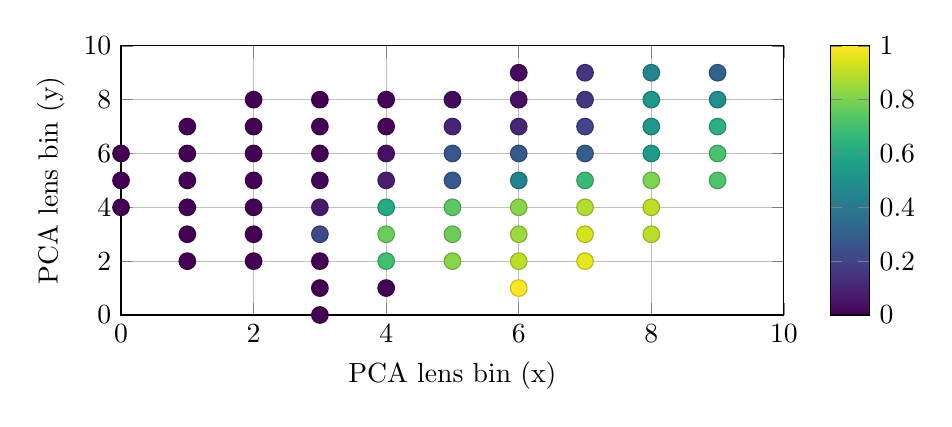
\begin{tikzpicture}\begin{axis}[width=10cm,height=5cm,xlabel={PCA lens bin (x)},ylabel={PCA lens bin (y)},colormap/viridis,colorbar,point meta min=0,point meta max=1,grid=major,xmin=0,xmax=10,ymin=0,ymax=10]
\addplot[scatter,only marks,mark=*,mark size=3pt,scatter src=explicit] coordinates {(0,4) [0.0] (0,5) [0.0] (0,6) [0.0] (1,2) [0.0] (1,3) [0.0] (1,4) [0.0] (1,5) [0.0] (1,6) [0.001] (1,7) [0.004] (2,2) [0.0] (2,3) [0.0] (2,4) [0.002] (2,5) [0.001] (2,6) [0.001] (2,7) [0.002] (2,8) [0.0] (3,0) [0.0] (3,1) [0.0] (3,2) [0.0] (3,3) [0.222] (3,4) [0.065] (3,5) [0.014] (3,6) [0.003] (3,7) [0.003] (3,8) [0.0] (4,1) [0.0] (4,2) [0.697] (4,3) [0.773] (4,4) [0.607] (4,5) [0.084] (4,6) [0.042] (4,7) [0.009] (4,8) [0.007] (5,2) [0.823] (5,3) [0.776] (5,4) [0.746] (5,5) [0.278] (5,6) [0.268] (5,7) [0.1] (5,8) [0.024] (6,1) [1.0] (6,2) [0.9] (6,3) [0.852] (6,4) [0.823] (6,5) [0.447] (6,6) [0.275] (6,7) [0.105] (6,8) [0.042] (6,9) [0.025] (7,2) [0.967] (7,3) [0.939] (7,4) [0.885] (7,5) [0.679] (7,6) [0.296] (7,7) [0.208] (7,8) [0.159] (7,9) [0.156] (8,3) [0.899] (8,4) [0.901] (8,5) [0.805] (8,6) [0.544] (8,7) [0.528] (8,8) [0.529] (8,9) [0.45] (9,5) [0.722] (9,6) [0.712] (9,7) [0.633] (9,8) [0.49] (9,9) [0.312]};
\end{axis}\end{tikzpicture}
\caption{\textbf{Mapper 2D positive-fraction scatter.} Dominant Mapper node per occupied PCA lens bin (largest node by membership), colored by positive fraction $\text{pos\_frac}$. The positive class localizes to a contiguous high-PC1 region (lens-$x \gtrsim 4$), peaking near bins $(6\text{--}8,\,1\text{--}4)$ at $>0.88$ positive fraction; low-PC1 bins (lens-$x \le 2$) are near-zero.}\label{fig:mapper}
\end{figure}

This spatial localization is consistent with the cross-family finding: frozen ESM-2 \cite{lin2023evolutionary} collects toxins from diverse Pfam families into one manifold region based on functional similarity ESM-2 learned from unsupervised pretraining, not based on explicit family signal. When a query lies near this cluster in cosine space, it gets positive-voted by residents of the cluster regardless of whether its actual family is represented; when a query lies far from the cluster (distant stratum), retrieval still pulls in cluster residents as nearest neighbors and inherits their positive labels with low accuracy.

\section{Biosecurity deployment consequence}
Panel expansion within the failing family is unlikely to be a rescue under the within-family-gap hypothesis tested here. A deployer who observes a distant-stratum false alarm in our regime should not assume that adding more toxin homologs from the failing family to the panel will fix it: in the 20 evaluable cases we examined, the failure was not caused by a gap in that family's representation; the embedding geometry itself was placing non-family neighbors near the query. Stronger conclusions await the 10-seed extension and a finer-grained family definition (InterPro superfamily, CATH fold) -- see Limitations.

Two actionable consequences follow:
\begin{enumerate}
\item Route every distant-stratum positive prediction to human review, regardless of vote count or $s_{\max}$. Calibration collapse (Paper 3) independently supports this rule.
\item Apply the panel-only learned linear projection (Paper 1) as preprocessing before retrieval. The projection improves distant $F_1$ from 0.120 to 0.177 at t30 $R{=}1000$ $k{=}25$, a 47\% relative rescue, by rotating the embedding space into a class-aware subspace. This addresses the correct mechanism: the cliff is a geometric property of the frozen embedding, not a gap in panel coverage.
\end{enumerate}

\section{Limitations}
(L1) Single seed analyzed (20260410). Extending to all 10 seeds is straightforward and unlikely to change the 100\% cross-family finding; deferred to v1.1.
(L2) 13\% of test proteins lack Pfam annotations and are excluded from the partition.
(L3) Within-family / cross-family as Pfam-ID overlap is a coarse family definition. A finer-grained analysis (InterPro superfamily, CATH fold, ECO level) could reveal distant-family-but-shared-superfamily relationships the crude Pfam test misses.
(L4) The result at $k=25$ may differ at $k=1$ where a single near-neighbor dominates.

\section{Data availability}
\texttt{data/results\_summaries/cross\_family\_partition.json} in this repository contains the per-case partition with query accession, query Pfam set, panel-voter Pfam union, and shared Pfam set for all 41 distant false alarms.

\bibliographystyle{unsrtnat}
\bibliography{references}
\end{document}
